\documentclass[a4paper, 10pt, garamond]{book}
\usepackage{cours-preambule}
\usepackage{tocloft}

% \renewcommand{\mtifont}{\large}
\renewcommand{\mtcSfont}{\Large}
\setlength{\mtcindent}{5pt}
\mtcsetoffset{minitoc}{-5pt}
% \mtcsetformat{minitoc}{tocrightmargin}{3em}
% \mtcsetformat{minitoc}{pagenumwidth}{-4em}
\addtolength{\cftsecnumwidth}{10pt}
% \mtcsetpagenumbers{minitoc}{off}
\makeatletter
% \renewcommand{\@pnumwidth}{-4em}
% \renewcommand{\@tocrmarg}{-0.5cm}
% \renewcommand{\cftdotsep}{\cftnodots}
\makeatother
\dominitoc
\faketableofcontents

% \toggletrue{student}
\HideSolutionstrue
\toggletrue{corrige}
% \renewcommand{\mycol}{black}
\renewcommand{\mycol}{gray}

\makeatletter
\renewcommand{\@chapapp}{MPSI3 -- 24 novembre 2023 -- Devoir surveillé}
\makeatother

\graphicspath{{./figures/}{./figures/E1}{./figures/E2}{./figures/P1}{./figures/P2}}

\newcommand{\figsvg}[1]{
  \begin{center}
    \subimport{figures/}{#1}
  \end{center}
}
\newcommand{\figsvgCap}[2]{
  \begin{center}
    \subimport{figures/}{#1}
    \captionof{figure}{#2}
  \end{center}
}

\begin{document}
\setcounter{chapter}{2}
\chapter{\cswitch{Correction du DS}{Oscillateurs et transformation de la
	  matière}}
\label{ch:ds03}

\enonce{
	\begin{center}
		\Large\bfseries
		Tout moyen de communication est interdit
		\smallbreak
		Les téléphones portables doivent être éteints et rangés dans les sacs
		\smallbreak
		\xul{Les calculatrices sont \textit{autorisées}}
	\end{center}
	\begin{tcb}*[cnt, bld](ror)<itc>{Au programme}
		\large
		Régimes transitoires d'ordre 2 (mécanique et électricité), transformation et
		équilibre chimique.
	\end{tcb}
	\vfill
	\minitoc
	\vfill

	Les différentes questions peuvent être traitées dans l'ordre désiré.
	\textbf{Cependant}, vous indiquerez le numéro correct de chaque question. Vous
	prendrez soin d'indiquer sur votre copie si vous reprenez une question d'un
	exercice plus loin dans la copie, sous peine qu'elle ne soit ni vue ni corrigée.
	\bigbreak
	Vous porterez une attention particulière à la \textbf{qualité de rédaction}.
	Vous énoncerez clairement les hypothèses, les lois et théorèmes utilisés. Les
	relations mathématiques doivent être reliées par des connecteurs logiques.
	\bigbreak
	Vous prendre soin de la \textbf{présentation} de votre copie, notamment au
	niveau de l'écriture, de l'orthographe, des encadrements, de la marge et du
	cadre laissé pour la note et le commentaire. Vous \textbf{encadrerez les
		expressions littérales}, sans faire apparaître les calculs. Vous ferez
	apparaître cependant le détail des grandeurs avec leurs unités. Vous
	\textbf{soulignerez les applications numériques}.
	\bigbreak
	Ainsi, l'étudiant-e s'expose aux malus suivants concernant la forme et le fond~:
	\begin{tcb}*(prop)"bomb"{Malus}
		\begin{minipage}[t]{0.50\linewidth}
			\begin{itemize}
				\item A~: application numérique mal faite~;
				\item N~: numéro de copie manquant~;
				\item P~: prénom manquant~;
				\item E~: manque d'encadrement des réponses~;
				\item M~: marge non laissée ou trop grande~;
				\item V~: confusion ou oubli de vecteurs~;
			\end{itemize}
		\end{minipage}
		\begin{minipage}[t]{0.50\linewidth}
			\begin{itemize}
				\item Q~: question mal ou non indiquée~;
				\item C~: copie grand carreaux~;
				\item U~: mauvaise unité (flagrante)~;
				\item H~: homogénéité non respectée~;
				\item S~: chiffres significatifs non cohérents~;
				\item $\f$~: loi physique fondamentale brisée.
			\end{itemize}
		\end{minipage}
	\end{tcb}

	\begin{tcb}(impo){Exemple application numérique}
		\vspace*{-10pt}
		\begin{minipage}[c]{0.45\linewidth}
			\begin{gather*}
				\boxed{n = \frac{PV}{RT}}
				\qav
				\left\{
				\begin{array}{rcl}
					p & = & \SI{1.0e5}{Pa}                \\
					V & = & \SI{1.0e-3}{m^3}              \\
					R & = & \SI{8.314}{J.mol^{-1}.K^{-1}} \\
					T & = & \SI{300}{K}
				\end{array}
				\right.\\
				\mathrm{A.N.~:}\quad
				\xul{n = \SI{5.6e-4}{mol}}
			\end{gather*}
		\end{minipage}
		\hfill
		\cancel{\bcancel{
				\begin{minipage}[c]{0.45\linewidth}
					\begin{gather*}
						n = \frac{PV}{RT} = \frac{\num{e5}\cdot\num{1}}{8.32\cdot300}
						= 0.56
					\end{gather*}
				\end{minipage}
			}}
	\end{tcb}
	\newpage
}

\setcounter{section}{0}
\exercice[30]{Pentachlorure de phosphore}
\resetQ
\enonce{
Le pentachlorure de phosphore \ce{PCl5} est un composé très toxique, servant
de réactif en synthèse organique pour ajouter des atomes de chlore à une
chaîne carbonée. Mis en phase gazeuse, il se décompose spontanément en
trichlorure de phosphore et en dichlore, donnant naissance à un équilibre en
phase gazeuse.

Considérons un réacteur fermé de volume constant $V = \SI{2}{L}$ maintenu à
température constante $T = \SI{180}{\celsius}$. À cette température, la
constante thermodynamique de l’équilibre précédemment cité vaut $K^\circ =
	8$. On y met $n_0 = \SI{0,5}{\mol}$ de \ce{PCl5}.

On rappelle que $R = \SI{8.314}{J.K^{-1}.mol^{-1}}$.
}

\QR[1]{%
	Exprimer puis calculer la pression initiale dans le réacteur $p_0$ en fonction
	des données.
}{%
	On applique la loi des gaz parfaits~:
	\begin{gather*}
		\boxed{p_0=\frac{n_0RT}{V}}
		\qav
		\left\{
		\begin{array}{rcl}
			n_0 & = & \SI{0.5}{mol}
			\\
			R   & = & \SI{8.314}{J.K^{-1}.mol^{-1}}
			\\
			T   & = & \SI{453.15}{K}
			\\
			V   & = & \SI{2e-3}{m^{3}}
		\end{array}
		\right.\\
		\AN
		\xul{
			p_0 = \SI{9.41e5}{Pa}
		}
	\end{gather*}
}

\QR[1]{%
	Écrire l’équation de réaction modélisant le processus dans le réacteur, et
	dresser le tableau d'avancement correspondant.
}{%
	\begin{center}
		\def\rhgt{0.35}
		\centering
		\begin{tabularx}{.7\linewidth}{|l|c||YdYdY||Y|}
			\hline
			\multicolumn{2}{|c||}{
				$\xmathstrut{\rhgt}$
			\textbf{Équation}}  &
			$\ce{PCl_5\gaz{}}$  & $=$                   &
			$\ce{PCl_3\gaz{}}$  & $+$                   &
			$\ce{Cl_2\gaz{}}$   &
			$n_{\tot, gaz}$                               \\
			\hline
			$\xmathstrut{\rhgt}$
			Initial             & $\xi = 0$             &
			$n_0$               & \vline                &
			$0$                 & \vline                &
			$0$                 &
			$n_0$                                         \\
			\hline
			$\xmathstrut{\rhgt}$
			Interm.             & $\xi$                 &
			$n_0 - \xi$         & \vline                &
			$\xi$               & \vline                &
			$\xi$               &
			$n_0 + \xi$                                   \\
			\hline
			$\xmathstrut{\rhgt}$
			Final               & $\xi_f = \xi\ind{eq}$ &
			$n_0 - \xi\ind{eq}$ & \vline                &
			$\xi\ind{eq}$       & \vline                &
			$\xi\ind{eq}$       &
			$n_0 + \xi\ind{eq}$                           \\
			\hline
		\end{tabularx}
	\end{center}
}

\QR[2]{%
	Exprimer les pressions partielles des gaz en fonction de $n_0$, $\xi$ et de la
	pression initiale $p_0$.
}{%
	On utilise à nouveau l'équation des gaz parfaits, avec $\frac{RT}{V} =
		\frac{p_0}{n_0}$~:
	\[
		\boxed{P_{\ce{PCl5}} = \frac{(n_0-\xi)RT}{V}=\frac{(n_0-\xi)p_0}{n_0}}
		\qqet
		\boxed{P_{\ce{PCl3}} = \frac{\xi p_0}{n_0}}
		\qqet
		\boxed{P_{\ce{Cl2}} = \frac{\xi p_0}{n_0}}
	\]
}

\QR[5]{%
	Exprimer le coefficient de dissociation à l’équilibre $\alpha = \xi\ind{eq}
		/n_0$ en fonction de $K^\circ $, $p^\circ $ et $p_0$. Faire l'application
	numérique. Que représente-t-il physiquement~?
}{%
	\noindent
	\begin{minipage}[t]{.5\linewidth}
		Loi d'action de masses~:
		\begin{DispWithArrows*}[fleqn, mathindent=10pt]
			K^\circ &=
			\eval{\frac{a(\ce{PCl3})a(\ce{Cl2})}{a(\ce{PCl5})}}\ind{eq}
			\Arrow{Activité d'un gaz}
			\\\Lra
			K^\circ &=
			\eval{
				\frac{\frac{P_{\ce{PCl3}}}{p^\circ}\frac{P_{\ce{Cl2}}}{p^\circ}}
				{\frac{P_{\ce{PCl5}}}{p^\circ}}}\ind{eq}
			\Arrow{Question 2}
			\\\Lra
			K^\circ &=
			\frac{\xi\ind{eq}^2}{n_0(n_0-\xi\ind{eq})}\frac{p_0}{p^\circ}
			\Arrow{On factorise}
			\\\Lra
			K^\circ &=
			\underbracket[1pt]{\cancel{\frac{n_0^{2}}{n_0^{2}}}}_{=1}
			\frac{\left( \frac{\xi\ind{eq}}{n_0} \right)^{2}}{1 \left(
				1-\frac{\xi\ind{eq}}{n_0} \right)}
			\frac{p_0}{p^\circ}
			\Arrow{$\alpha = \xi\ind{eq}/n_0$}
			\\\Lra
			K^\circ &=
			\frac{\alpha^2}{(1-\alpha)}\frac{p_0}{p^\circ }
		\end{DispWithArrows*}
	\end{minipage}
	\hfill
	\begin{minipage}[t]{.5\linewidth}
		Ainsi, en isolant~:
		\begin{DispWithArrows*}
			\alpha^2 &+ \alpha\left(\frac{K^\circ p^\circ }{p_0} \right) -
			\frac{K^\circ p^\circ }{p_0} = 0
			% \Arrow{$\Delta$ son discriminant}
			\\\Ra
			\Delta &=
			\left(\frac{K^\circ p^\circ }{p_0} \right)^2 +
			4\left(\frac{K^\circ p^\circ }{p_0} \right) > 0
			% \Arrow{Solution positive}
			\\\Lra
			\Aboxed{
				\alpha &= -\left(\frac{K^\circ p^\circ }{2p_0} \right) +
				\sqrt{\left(\frac{K^\circ p^\circ }{2p_0} \right)^2 +
					\left(\frac{K^\circ p^\circ }{p_0} \right)}}
			\\\Ra
			\makebox[0pt][l]{$\phantom{\AN}\xul{\phantom{\alpha = \num{0.59}}}$}
			\AN
			\alpha &= \num{0.59}
		\end{DispWithArrows*}
		$\alpha$ représente la proportion de réactif ayant effectivement réagit.
	\end{minipage}
}

\QR[2]{%
	Calculer la pression régnant dans le réacteur à l’équilibre.
}{%
	À l'aide du tableau d'avancement, on a $n\ind{tot, gaz}$, d'où

	\begin{gather*}
		P\ind{eq} = \frac{n_0+\xi\ind{eq}}{n_0}p_0
		\Lra
		\boxed{
			P\ind{eq} = (1+\alpha)p_0
		}
		\\
		\AN
		\xul{P\ind{eq} = \SI{15,0}{bar}}
	\end{gather*}
}

\resetQ
\exercice[30]{États finaux variés}
\enonce{
	On s'intéresse dans un premier temps à une solution aqueuse obtenue à
	\SI{298}{K} par un mélange d'acide éthanoïque \ce{CH3COOH} (concentration
	$c_1=\SI{0.10}{mol.L^{-1}}$ après mélange) et d'ions fluorure \ce{F-}
	(concentration $c_2=\SI{5.0e-2}{mol.L^{-1}}$ après mélange).
	La réaction \eqref{eq:R1} susceptible de se produire s'écrit~:
	\begin{alignat}{2}
		\ce{CH3COOH(aq) + F^-(aq) & = CH3COO^-(aq) & + HF(aq)}
		\tag{1}\label{eq:R1}
		\\
		\intertext{On connaît les constantes d'équilibre à \SI{298}{K} des réactions
			suivantes~:}
		\beforetext{$K^\circ_2 = \num{e-4.8}$}
		\ce{CH3COOH(aq) + H2O     & = CH3COO^-(aq) & + H3O^+(aq)}
		\tag{2}\label{eq:R2}
		\\
		\beforetext{$K^\circ_3 = \num{e-3.2}$}
		\ce{HF(aq) + H2O          & = F^-(aq)      & + H3O^+(aq)}
		\tag{3}\label{eq:R3}
	\end{alignat}
}

\QR[1]{%
	Calculer la constante d'équilibre $K^\circ_1$ relative à
	l'équilibre~\eqref{eq:R1}.
}{%
	On constate que l'équilibre%
	\sswitch{%
		$(1) = (2) - (3)$
	}{%
		$\eqref{eq:R1}=\eqref{eq:R2}-\eqref{eq:R3}$
	}%
	donc
	\[
		\boxed{K^\circ_1=\cfrac{K^\circ_2}{K^\circ_3}=\num{e-1.6}}
	\]
}

\QR[4]{%
	Déterminer l'état d'équilibre de la solution issue du mélange de l'acide
	éthanoïque et des ions fluorure~: exprimer l'équation dont l'avancement est
	solution, et l'expression littérale de la solution en fonction de $c_1$, $c_2$
	et $K_1^\circ$.
}{%
	On dresse le tableau d'avancement en concentration~:
	\begin{center}
		\def\rhgt{0.35}
		\centering
		\begin{tabularx}{\linewidth}{|l|c||YdYdYdY|}
			\hline
			\multicolumn{2}{|c||}{
				$\xmathstrut{\rhgt}$
			\textbf{Équation}}        &
			$\ce{CH_3COOH(aq)}$       & $+$               &
			$\ce{F^{-}(aq)}$          & $\ra$             &
			$\ce{CH_3COO^{-}(aq)}$    & $+$               &
			$\ce{HF(aq)}$                                   \\
			\hline
			$\xmathstrut{\rhgt}$
			Initial                   & $x = 0$           &
			$c_1$                     & \vline            &
			$c_2$                     & \vline            &
			$0$                       & \vline            &
			$0$                                             \\
			\hline
			$\xmathstrut{\rhgt}$
			Interm.                   & $x$               &
			$c_1 - x$                 & \vline            &
			$c_2 - x$                 & \vline            &
			$x$                       & \vline            &
			$x$                                             \\
			\hline
			$\xmathstrut{\rhgt}$
			Final ($\si{mol.L^{-1}}$) & $x_f = x\ind{eq}$ &
			$\num{9.0e-2}$            & \vline            &
			$\num{4.0e-2}$            & \vline            &
			$\num{9.6e-3}$            & \vline            &
			$\num{9.6e-3}$                                  \\
			\hline
		\end{tabularx}
	\end{center}

	D'après la loi d'action de masse,
	\begin{DispWithArrows*}[groups]
		K^\circ_1 &= \cfrac{x\ind{eq}^2}{(c_1-x\ind{eq})\times (c_2-x\ind{eq})}
		\Arrow{On isole}
		\\\Lra
		(c_1-x\ind{eq})(c_2-x\ind{eq})K^\circ_1 &= x\ind{eq}^{2}
		\Arrow[new-group]{On rassemble}
		\\\Lra
		x\ind{eq}^{2} + (x\ind{eq}-c_1)(x\ind{eq}-c_2)K^\circ_1 &= 0
		\Arrow{On développe et factorise}
		\\\Lra
		\Aboxed{
			x\ind{eq}^{2}(1+K^\circ_1) -
			x\ind{eq}(c_1+c_2)K^\circ_1 + c_1c_2K^\circ_1 &= 0
		}
	\end{DispWithArrows*}
	Ainsi, avec $\Delta$ le discriminant de ce trinôme~:
	\begin{DispWithArrows*}
		\Delta &= \left( c_1+c_2 \right)^{2}\left( K_1^\circ \right)^{2}
		-4(1+K_1^\circ)c_1c_2K_1^\circ
		\Arrow{Solutions}
		\\\Ra
		\Aboxed{
			x_{\equ,\pm} &=
			\frac{
				(c_1+c_2)K_1^\circ \pm \sqrt{
					\left( c_1+c_2 \right)^{2}\left( K_1^\circ \right)^{2}
					-4(1+K_1^\circ)c_1c_2K_1^\circ}
			}{2(1+K_1^\circ)}
		}
		\Arrow{Calcul}
		\\
		\makebox[0pt][l]{%
			$\phantom{\AN}\xul{\phantom{x\ind{eq} = \SI{9.6e-3}{mol.L^{-1}}}}$%
		}
		\AN
		x\ind{eq} &= \SI{9.6e-3}{mol.L^{-1}}
		\qav
		\left\{
		\begin{array}{rcl}
			c_1       & = & \SI{0.1}{mol.L^{-1}}
			\\
			c_2       & = & \SI{5.0e-2}{mol.L^{-1}}
			\\
			K_1^\circ & = & \num{e-1.6}
		\end{array}
		\right.
	\end{DispWithArrows*}
	On en déduit les concentrations à l'équilibre indiquées dans le tableau.
}

\enonce{
	On étudie dans la suite de l'exercice quelques constituants du béton.
	L'hydroxyde de calcium \ce{Ca(OH)_2(s)} confère au béton ses propriétés
	basiques (au sens de acide ou base). Il se dissout en solution aqueuse selon
	la réaction~\eqref{eq:R4}~:
	\begin{gather}
		\beforetext{$K^\circ_4(\SI{298}{K}) = \num{e-5.2}$}
		\ce{Ca(OH)_2(s) = Ca^{2+}(aq) + 2HO^-(aq)}
		\tag{4}\label{eq:R4}
	\end{gather}
}

\QR[3]{%
	On introduit en solution aqueuse un net excès d'hydroxyde de calcium. La phase
	solide est alors présente en fin d'évolution. Calculer les concentrations de
	chacun des ions présents à l'équilibre.
}{%
	On dresse un tableau d'avancement en concentration~:
	\begin{center}
		\def\rhgt{0.35}
		\centering
		\begin{tabularx}{.7\linewidth}{|l|c||YdYdY|}
			\hline
			\multicolumn{2}{|c||}{
				$\xmathstrut{\rhgt}$
			\textbf{Équation}}        &
			$\ce{Ca(OH)2(s)}$         & $=$               &
			$\ce{Ca^{2+}(aq)}$        & $+$               &
			$2\ce{HO^{-}(aq)}$                              \\
			\hline
			$\xmathstrut{\rhgt}$
			Initial                   & $x = 0$           &
			excès                     & \vline            &
			$0$                       & \vline            &
			$0$                                             \\
			\hline
			$\xmathstrut{\rhgt}$
			Interm.                   & $x$               &
			excès                     & \vline            &
			$x$                       & \vline            &
			$2x$                                            \\
			\hline
			$\xmathstrut{\rhgt}$
			Final ($\si{mol.L^{-1}}$) & $x_f = x\ind{eq}$ &
			excès                     & \vline            &
			$\num{1.2e-2}$            & \vline            &
			$\num{2.4e-2}$                                  \\
			\hline
		\end{tabularx}
	\end{center}
	\begin{gather*}
		\beforetext{Par la loi d'action de masse,}
		K^\circ_4=x\ind{eq}\times (2x\ind{eq})^2
		\qdonc
		\boxed{x\ind{eq}=\pa{\cfrac{K^\circ_4}{4}}^{1/3}}
		\\\AN
		\xul{x\ind{eq}=\SI{1.2e-2}{mol.L^{-1}}}
	\end{gather*}
	On en déduit les concentrations indiquées dans le tableau.
}

\QR[1]{%
	On donne la relation $[\ce{H_3O+}][\ce{HO^{-}}] = \num{e-14}$. Sachant que $\pH
		= -\log([\ce{H_3O^{+}}])$, déterminer le $\pH$ de la solution. Le milieu
	est-il acide, basique ou neutre~?
}{%
	\[
		\boxed{\pH =14+\log[\ce{HO-}]}
		\Ra
		\xul{\pH = \num{12,4}}
	\]
	ce qui corrspond bien à un milieu basique.
}

\enonce{
	Dans certains cas, la pollution urbaine liée à l'humidité entraine la
	dissolution du dioxyde de carbone atmosphérique dans l'eau à l'intérieur du
	béton (sous forme \ce{H2CO3}), provoquant la carbonatation du béton (formation
	de carbonate de calcium \ce{CaCO_3(s)}) par réaction de l'hydroxyde de calcium
	\ce{Ca(OH)_2(s)} avec la forme \ce{H2CO_3(aq)}.
}

\QR[2]{%
	Écrire la réaction $(5)$ mise en jeu dans la carbonatation du béton et calculer
	sa constante d'équilibre $K^\circ_5$ à \SI{298}{K}. On donne à \SI{298}{K} les
	constantes d'équilibre des réactions suivantes~:
	\begin{alignat}{2}
		\beforetext{$K^\circ_6=\num{e-8.4}$}
		\ce{CaCO_3(s)         & = Ca^{2+}(aq)   & + CO^{2-}_3(aq)}
		\tag{6}\label{eq:R6}
		\\
		\beforetext{$K^\circ_7=\num{e-6.4}$}
		\ce{H2CO_3(aq) + H2O  & = HCO^-_3(aq)   & + H3O^+(aq)}
		\tag{7}\label{eq:R7}
		\\
		\beforetext{$K^\circ_8=\num{e-10.3}$}
		\ce{HCO^-_3(aq) + H2O & = CO^{2-}_3(aq) & + H3O^+(aq)}
		\tag{8}\label{eq:R8}
		\\
		\beforetext{$K^\circ_9=\num{e-14}$}
		\ce{2H2O              & = HO^-(aq)      & + H3O^+(aq)}
		\tag{9}\label{eq:R9}
	\end{alignat}
}{%
	\ifstudent{
		\vspace*{-\dimexpr\baselineskip+\abovedisplayskip\relax}
	}
	\begin{gather}
		\beforetext{On écrit la réaction~\eqref{eq:R5}~:}
		% \beforetext{$K^\circ_5$}
		\ce{Ca(OH)_2(s) + H2CO_3(aq) = CaCO_3(s) + 2H2O}
		\tag{5} \label{eq:R5}
	\end{gather}
	On constate que la réaction
	\sswitch{%
		$(5)=(4)-(6)+(8)+(7)-2\times(9)$
	}{%
		$\eqref{eq:R5} = \eqref{eq:R4} - \eqref{eq:R6} + \eqref{eq:R8} +
			\eqref{eq:R7} -2\eqref{eq:R9}$
	}%
	donc
	\[
		\boxed{
			K^\circ_5 =
			\cfrac{K^\circ_4K^\circ_7K^\circ_8}
			{K^\circ_6(K^\circ_9)^2}
			= \num{e14.5}
		}
	\]
}

\enonce{
	On étudie désormais la réaction de décomposition du carconate de calcium
	\ce{CaCO_3(s)} en oxyde de calcium \ce{CaO(s)} et dioxyde de carbone
	\ce{CO_2(g)} de constante d'équilibre $K^\circ=0,20$ à \SI{1093}{K}.
	\[
		\ce{CaCO_3(s) = CaO(s) + CO2(g)}
	\]
	Soit un récipient indéformable de volume $V=\SI{10}{L}$, vidé au préalable de
	son air, et maintenu à la température constante de \SI{1093}{K}. On introduit
	progressivement une quantité de matière $n$ en carbonate de calcium solide et
	on mesure la pression $p$ à l'intérieur de l'enceinte.
}

\QR[2]{%
Lorsque l'équilibre est établi, calculer la quantité de matière en dioxyde de
carbone $n(\ce{CO2})\ind{eq}$ dans l'enceinte. On supposera les gaz comme
parfaits. On rappelle la constante des gaz parfaits
$R=\SI{8,31}{J.K^{-1}.mol^{-1}}$.
}{%
À l'équilibre, d'après la loi d'action de masse,
\begin{DispWithArrows*}[groups]
	K^\circ &= \cfrac{P(\ce{CO2})\ind{eq}}{P^\circ}
	\Arrow{$\DS P (\ce{CO_2})\ind{eq} = \frac{n(\ce{CO_2})\ind{eq}RT}{V}$}
	\\\Lra
	K^\circ &= \frac{n(\ce{CO_2})\ind{eq}RT}{VP^\circ}
	\Arrow{On isole}
	\\\Lra
	\Aboxed{n(\ce{CO2})\ind{eq} &= \cfrac{K^\circ P^\circ V}{RT}}
	\\
	\makebox[0pt][l]{%
		$\phantom{\AN}\xul{\phantom{n(\ce{CO_2})\ind{eq} = \SI{2.2e-2}{mol}}}$%
	}
	\AN n(\ce{CO_2})\ind{eq} &= \SI{2.2e-2}{mol}
	\qav
	\left\{
	\begin{array}{rcl}
		K^\circ & = & \num{0.20}
		\\
		P^\circ & = & \SI{1e5}{Pa}
		\\
		V       & = & \SI{10e-3}{m^{3}}
		\\
		R       & = & \SI{8.314}{J.K^{-1}.mol^{-1}}
		\\
		T       & = & \SI{1093}{K}
	\end{array}
	\right.
\end{DispWithArrows*}
}

\QR[2]{%
	On introduit une quantité de matière $n=\SI{1.0e-2}{mol}$ en carbonate de
	calcium. Décrire l'état final. On précisera notamment si l'état final est un
	état d'équilibre.
}{%
	Comme $n<n(\ce{CO2})\ind{eq}$, le quotient réactionnel évoluera de sa valeur
	initiale 0 jusqu'à sa valeur maximale $Q\ind{max}$, qui sera inférieure à
	$K^\circ$. Ainsi la réaction évoluera dans le sens direct jusqu'à
	\textbf{disparition complète} du carbonate de calcium~: c'est une
	\textbf{rupture d'équilibre}.
	\smallbreak
	Les quantités de matière sont~:
	\[
		\xul{
			n(\ce{CO2})_f=n(\ce{CaO})_f=n=\SI{1.0e-2}{mol}
		}
		\qet
		\xul{
			n(\ce{CaCO3})_f=0
		}
	\]
}

\QR[2]{%
	Reprendre la question précédente dans le cas où $n=\SI{5.0e-2}{mol}$.
}{%
	Comme $n>n(\ce{CO2})\ind{eq}$, le quotient réactionnel peut augmenter jusqu'à
	atteindre la constante d'équilibre. L'état final est donc \textbf{bien un état
		d'équilibre} avec
	\begin{gather*}
		\boxed{n(\ce{CO2})_f=n(\ce{CaO})_f=n(\ce{CO2})\ind{eq}=\SI{2.2e-2}{mol}}
		\\
		\boxed{n(\ce{CaCO3})_f=n-n(\ce{CO2})\ind{eq}=\SI{2.8e-2}{mol}}
	\end{gather*}
}

\QR[1]{%
	Montrer que la courbe $p=f(n)$, avec $p$ la pression à l'intérieur de
	l'enceinte, est constituée de deux segments de droites dont on donnera les
	équations pour $0\leq n\leq\SI{0.10}{mol}$.
}{%
	On utilise les résultats précédents en appliquant l'équation d'état des gaz
	parfaits~:
	\begin{itemize}
		\item $n<n(\ce{CO2})\ind{eq} \Ra p = \cfrac{nRT}{V} \propto n$~;
		\item $n\geq n(\ce{CO2})\ind{eq} \Ra p = \cfrac{n(\ce{CO2})\ind{eq}RT}{V}
			      =\cte$.
	\end{itemize}
}

\setcounter{section}{0}
\resetQ
\prblm[49]{Amortissement et facteur de qualité d'un circuit RLC}
\enonce{
	On considère le circuit RLC série représenté ci-dessous.
	\begin{figure}[htbp]
	  \centering
	  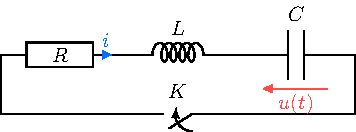
\includegraphics[width=.5\linewidth]{rlc_descendant}
	  \caption{Circuit.}
	  \label{fig:P1base}
	\end{figure}
  L'interrupteur $K$ est fermé à un instant $t=0$ choisi comme origine des
  temps. Le condensateur est initialement chargé~: $u(t=0)=u_0$.
}

\QR{

  Établir l'équation différentielle vérifiée par $u(t)$ pour $t\geq 0$. La
  mettre sous la forme
  \[
    \dv[2]{u}{t} + \frac{\w_0}{Q}\dv{u}{t} + \w_0{}^{2}u = 0
  \]
  et donner les expressions de $\w_0$ et $Q$ en fonction de $R$, $L$ et $C$.

}{
	Pour $t\geq 0$, l'interrupteur $K$ est fermé.

	Loi des mailles :
	\eq{
		u + u_R + u_L = 0
	}
	Relations pour les composants (convention récepteur) :

	$u_R = R i$ ; $ \qquad u_L = L\dv{i}{t} $ ;   $ \qquad i = C \dv{u}{t} $

	En utilisant les relations précédentes et en remplaçant dans la loi des mailles :
	\eq[equation]{ \label{equadiff}
		LC\dv[2]{u}{t} + RC\dv{u}{t} + u =0
	}
	Posons $\w_0=\dfrac{1}{\sqrt{LC}}$ et $Q=\dfrac{1}{R}\sqrt{\dfrac{L}{C}}$, nous obtenons :
	\eq{
		\boxed{ \dv[2]{u}{t} + \dfrac{\w_0}{Q} \dv{u}{t} + \w_0^2 u = 0 }
	}
	\begin{itemize}
		\item Si $ Q > \frac{1}{2} $, le régime est \emph{pseudo-périodique},
		\item si $Q < \frac{1}{2}$ le régime est \emph{apériodique},
		\item si $Q = \frac{1}{2}$ le régime est \emph{critique}.
	\end{itemize}
}
\QR{%
  Montrer que le système répond différemment selon la valeur de $Q$. Nommer
  chaque régime possible, sans chercher à donner les formes de solutions
  correspondantes.
}{%
  solu
}

\enonce{
	On suppose $Q >1/2$ dans la suite.
}

\begin{blocQR}
	\item
	\QR{
    Définir la pseudo-pulsation $\W$ des oscillations libres en fonction de
    $\w_0$ et $Q$. Définir aussi le temps caractéristique d'amortissement des
    oscillations libres en fonction de $\w_0$ et $Q$.
	}{
    Les résultats ont été obtenus en cours (écrire l'équation caractéristique
    associée à l'équation différentielle puis chercher les solutions complexes
    conjugués) :

		\eq{
			\boxed{\w = \w_0\sqrt{1 - \frac{1} {4Q^2}}} \qquad \boxed{\tau = \frac{2Q}{\w_0}}
		}
		% L'énoncé attend sans doute le temps de relaxation $\tau = \frac{Q}{\w_0}$ mais la forme canonique en $\dv[2]{u}{t} + \dfrac{1}{\tau} \dv{u}{t} + \w_0^2 u = 0$ n'est pas à connaître. 

	}

	\QR{
    Établir l'expression de $u(t)$ pour $t\geq 0$, compte tenu des conditions
    initiales que vous expliciterez et justifierez.
	}{
		Comme $Q >1/2$, le régime est pseudo-périodique et $u(t)$ est de la forme $u(t) = e^{-\frac{ t}{\tau}} \left( A \cos{(\w t)} + B \sin{(\w t)} \right) $ avec $\w$ la pseudo-pulsation.

		$A$ et $B$ sont des constantes à déterminer à l'aide des conditions initiales.

		D'après l'énoncé, le condensateur est initialement chargé sous la tension $u(t = 0^-) = u_0=u(t=0^+)$ donc $A = u_0$. (Pas de discontinuité de tension aux bornes du condensateur).

		Aucun courant ne circulait dans le circuit pour $t <0$ (interrupteur $K$ ouvert). Comme il n'y a pas de discontinuité du courant traversant la bobine, on en déduit $i(0^+)=i(0^-)=0$. Ainsi : $ \dv*{u}{t}{0^+} = 0$ d'où $B = \dfrac{\w_0 u_0}{2Q\w}$.
	}
\end{blocQR}


\enonce{
	On souhaite visualiser la tension $u(t)$ sur l'écran d'un oscilloscope dont l'entrée est modélisée par l'association en parallèle d'une résistance $R_0=\SI{1,0}{\mega \ohm}$ et d'une capacité $C_0=\SI{11}{\pico \farad}$.
}

\begin{blocQR}
	\item
	\QR{
		Montrer que si l'on tient compte de l'oscilloscope, l'équation différentielle vérifiée par $u(t)$ devient:
		\eq{
			L(C+C_0)\dv[2]{u}{t }+\left(\frac{L}{R_0}+RC+RC_0\right)\dv{u}{t}+\left(1+\frac{R}{R_0}\right)u=0
		}
	}{
		On commence par représenter le circuit en ajoutant en parallèle de $C$ la résistance $R_0$ et la capacité $C_0$.
		\begin{figure}[htbp!]
		  \centering
		  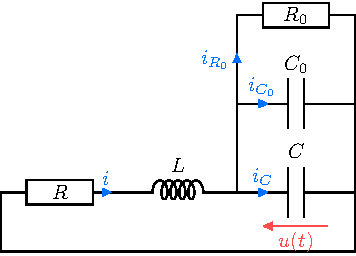
\includegraphics[width=.5\linewidth]{rlc_oscillo}
		  \caption{Circuit avec oscilloscope.}
		  \label{fig:P1osci}
		\end{figure}

		Loi des noeuds : $i = i_{R0} + i_{C0} + i_C$

		Relations pour les composants (convention récepteur) :

		$ u_R = R i $ ; $\qquad 	u_L = L\dv{i}{t} $ ; $\qquad i_C = C \dv{u}{t} $; $\qquad i_{C0} = C_0 \dv{u}{t} $ ; $\qquad u = R_0 i_{R0} $

		Remplaçons $i_C$, $i_{C0}$ et $i_{R0}$ dans la loi des noeuds, nous obtenons : $ i = \frac{u}{R_0} + (C+C_0)\dv{u}{t}$.

		Loi des mailles :
		\eq{
			u + u_R + u_L = 0 \qquad \text{soit} ~~ u + Ri + L\dv{i}{t} = 0
		}
		En remplaçant $i$, nous obtenons bien :
		\eq{
			L(C+C_0)\dv[2]{u}{t }+\left(\frac{L}{R_0}+RC+RC_0\right)\dv{u}{t}+\left(1+\frac{R}{R_0}\right)u=0
		}
	}

	\QR{
		Quelles relations qualitatives doivent vérifier $R$, $L$, $C$, $R_0$ et $C_0$ pour que la mise en place de l'oscilloscope ait une influence négligeable sur les oscillations étudiées~? Vérifier qu'avec les valeurs usuelles de $R$, $L$ et $C$ utilisées en travaux pratiques ces relations sont vérifiées.
	}{
		Pour que l'oscilloscope ait le moins d'influence possible sur les oscillations, il faut que les coefficients de l'équation différentielle précédente diffèrent le moins possible de ceux de l'équation différentielle (\ref{equadiff}) :

		\begin{itemize}
			\item $C >> C_0$; les capacités utilisées en T.P. sont de l'ordre du $\si{\nano \farad}$ ou du $\si{\micro \farad}$. Comme $C_0=\SI{11}{\pico \farad}$, cette condition est bien vérifiée ;
			\item $R << R_0$; les résistances utilisées en T.P sont de l'ordre du $\si{\kilo \ohm}$. Comme  $R_0=\SI{1,0}{\mega \ohm}$ , cette condition est bien vérifiée ;
			\item $\frac{L}{R_0} << RC$ soit $R_0 >> \frac{L}{RC} \approx \frac{10^{-2}}{10^3.10^{-9}} = 10^4 \w$; cette condition est bien vérifiée.
		\end{itemize}
	}

	\QR{
		On définit le décrément logarithmique comme étant la quantité $d_m=\ln\dfrac{u(t)}{u(t+mT)}$ où $T=2\pi/\w$ et $m$ est un entier strictement positif. Exprimer $d_m$ en fonction de $m$ et de $Q$.
	}{
		En remarquant que $ \cos{(\w (t + T))} = \cos{(\w t + 2\pi)} = \cos{(\w t)}$, on montre facilement que $d_m =\ln { \left( \exp{\frac{\w_0 m T}{2Q}} \right) }$.

		On obtient donc : $d_m = \dfrac{\w_0 m T}{2Q}$. En remplaçant $T$ par $\frac{2\pi}{\w}$ où $\w = \w_0 \sqrt{1 - \frac{1} {4Q^2}}$, il vient :
		\eq{
			\boxed{d_m = \frac{2 \pi m}{\sqrt{4Q^2-1}}}
		}
	}

	\QR{
		On réalise un montage expérimental où le circuit RLC est excité par un générateur BF. Comment faut-il choisir le signal délivré par le générateur pour observer les oscillations libres du circuit? La tension aux bornes du condensateur est enregistrée gr\^ace à un logiciel d'acquisition. Le signal obtenu est représenté sur la figure ci-dessous.
		\begin{figure}[htbp!]
		  \centering
		  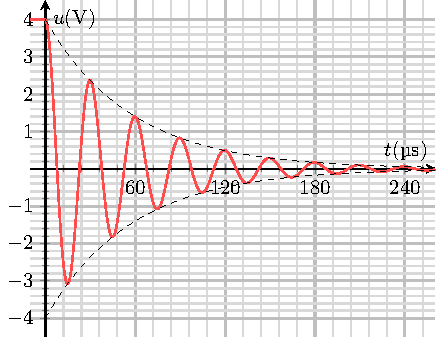
\includegraphics[width=.8\linewidth]{carac-rlc-15}
		  \caption{Signal obtenu.}
		  \label{fig:P1sign}
		\end{figure}
		Estimer le facteur de qualité $Q$ du circuit.
	}{
		Pour observer les oscillations il faut que la demi-période du signal délivré par le G.B.F. soit égale à quelques $\tau$. \\

		On lit graphiquement $u(0)=4,0$V et $u(2T)=1,4$V. On peut alors calculer $d_2=\ln\dfrac{u(0)}{u(2T)}$.

		Comme $d_2= \frac{4 \pi }{\sqrt{4Q^2-1}}$, on en déduit : $\boxed{ Q = \sqrt{ \frac{1}{4} + 4 \left( \frac{\pi}{d_2} \right) ^2} }$. Application numérique : $ \underline{Q = 6,0}$
	}
\end{blocQR}

\enonce{
	On suppose $Q\gg 1$: la dissipation d'énergie par effet Joule est traitée comme une perturbation par rapport au cas du circuit non dissipatif ($R=0$).
}

\begin{blocQR}
	\item
	\QR{
		Dans le cas où $R=0$, établir l'expression de la valeur moyenne temporelle $\langle {\cal E}\rangle$ de l'énergie électromagnétique stockée dans le circuit.
	}{
		Dans le cas où $R = 0$, le circuit est non dissipatif donc l'énergie emmagasinée dans le condensateur et la bobine reste constante.

		Évaluons l'énergie initiale (pas de courant dans la bobine) :  $ {\cal E}(t = 0) = \frac{Cu_0^2}{2}$.

		Ainsi : $ \boxed{ <{\cal E}> = \frac{Cu_0^2}{2} }$
	}

	\QR{
	Dans le cas où $R\neq 0$, montrer qu'au premier ordre en $1/Q$, l'énergie $W_J$ dissipée par effet Joule dans le circuit RLC, pendant une pseudo-période, vérifie la relation:
	\eq{
		W_J = \frac{2\pi}{Q}\langle {\cal E}\rangle
	}
	}{
	Il faut évaluer l'énergie emmagasinée par le condensateur et la bobine à l'instant $t$ :
	\eq{
		{\cal E}(t) = \frac{Cu^2(t)}{2} + \frac{Li^2(t)}{2}
	}


	Pour $Q >> 1$, on a $\w \approx \w_0$ , l'expression de $u(t)$ devient :
	\eq[align*]{
		u(t) &= u_0 e^{-\frac{t}{\tau}} \left( \cos{(\w t)} + \frac{\w_0}{2Q\w} \sin{(\w t)} \right) \\
		& \approx u_0 e^{-\frac{t}{\tau}} \left( \cos{(\w_0 t)} + \frac{1}{2Q} \sin{(\w_0 t)} \right) \\
		u(t)  & \approx u_0 e^{-\frac{t}{\tau}}  \cos{(\w_0 t)}
	}
	On calcule alors : $ i(t) = C \dv{u}{t} $ :
	\eq[align*]{
		i(t) &= -Cu_0 e^{-\frac{t}{\tau}} \left( \w_0 \sin{(\w_0 t)} + \frac{1}{\tau}  \cos{(\w_0 t)} \right) \\
		i(t)  & \approx -Cu_0 \w_0 \sin{(\w_0 t)} e^{-\frac{t}{\tau}}
	}
	En effet, $ \frac{1}{\tau} = \frac{\w_0}{2Q} << \w_0$ pour $Q >>1$.

	On calcule alors $ {\cal E}(t) = \frac{Cu^2(t)}{2} + \frac{Li^2(t)}{2}$, il vient :
	\eq{
		{\cal E}(t) = \frac{1}{2} C u_0^2 e^{ -\frac{2t}{\tau} }
	}

	En une pseudo-période $T$, l'énergie décroît de la quantité :
	\eq{
	{\cal E}(t) - {\cal E}(t+T) = \frac{1}{2} C u_0^2 e^{ -\frac{2t}{\tau} } \left( 1 - e^{ -\frac{2T}{\tau} } \right)
	}
	On a $ e^{ -\frac{2T}{\tau} } = e^{ -\frac{\w_0 T}{Q} } \approx e^{ -\frac{2 \pi}{Q} } $ (car $\w \approx \w_0$).

	Pour $Q >> 1$, avec un développement limité à l'ordre 1, on a : $ 1 - e^{ -\frac{2 \pi}{Q} } \approx 1 - 1 + \frac{2 \pi}{Q}$.

	L'énergie dissipée par effet Joule en une pseudo-période correspond à l'énergie perdue par $L$ et $C$ pendant cette durée donc $W_J = {\cal E}(t) - {\cal E}(t+T) $.

	Nous obtenons bien :
	\eq{
		\boxed{W_J \approx \frac{2\pi <{\cal E}>}{Q}}
	}

	}
\end{blocQR}

\resetQ
\prblm[30]{Modélisation des mouvements d'une plateforme offshore}
\enonce{
On s’intéresse à la résolution d’une équation du mouvement dans une approche classique de la mécanique afin d’étudier le mouvement simplifié d’une plateforme en mer. Le modèle envisagé est un système à un degré de liberté considéré comme un oscillateur harmonique : une masse est reliée à un ressort, avec amortissement.

On considère le mouvement d’une plateforme en mer soumise à un courant marin. Sa partie supérieure de masse $m = \SI{110}{tonnes}$ est considérée comme rigide et le mouvement principal de la plateforme a lieu suivant $x$ (cf figure 1(a)). Afin d’étudier le mouvement de cette plateforme, on la représente par une masse $m$, liée à un ressort de 
constante de raideur $k$ et à un amortisseur de constante d’amortissement $\gamma$ comme schématisé sur la figure 1(b). 
La masse se déplace selon une seule direction, parallèle à l’axe $Ox$ en fonction du temps $t$. Ainsi, les projections sur l’axe $Ox$ de la position, de la vitesse et de l’accélération de la masse en fonction du temps sont notées respectivement $x(t)$, $\dot{x}(t)$ et $\ddot{x}(t)$. Le vecteur unitaire de l’axe $Ox$ est noté $\vec{i}$.

\begin{figure}[htbp!]
  \centering
  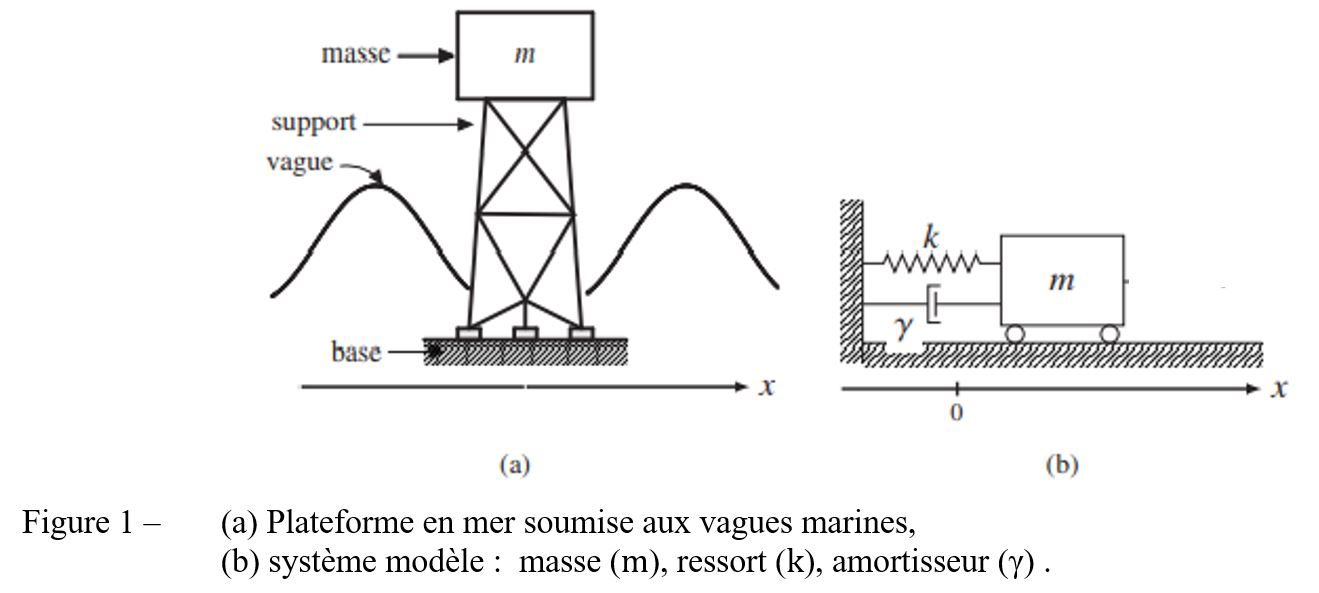
\includegraphics[width=.9\linewidth]{P2base}
\end{figure}

La masse se déplace sur la base horizontale sans frottements sur le support. La position d’équilibre de la masse sera choisie à $x = 0$.

La force totale $\vec{F_{tot}}$ agissant sur la masse correspond à la réaction normale à la base horizontale $\vec{R_N}$, à la force de frottement $\vec{F_d}= - \gamma \vec{v}$  où $\gamma$ est la constante d’amortissement positive, permettant  de prendre en compte l’effet de l’eau environnante, à la force de rappel $\vec{F_k}$ du ressort et au poids $\vec{P}$ de la masse $m$.
}

\QR
{Etablir l’équation différentielle du mouvement de la masse $m$ et la mettre sous la forme :

\centersright{$\ddot{x}+2\xi\w_0 \dot{x}+{\w_0}^2 x=0$}{(équation 1)}

\noindent
On exprimera $\w_0$ et $\xi$ en fonction de $k$, $m$ et $\gamma$. On rappelle que $\xi =Q/2$.}
{
\begin{itemize}
\item Référentiel d'étude: Référentiel terrestre $\mathcal{R}(O, x, y)$ supposé galiléen.
\item Base de projection : Base cartésienne $(O, x, y)$ de vecteurs unitaires $\vec{i}$ et $\vec{j}$. L'origine est prise à la position d'équilibre comme indiqué dans l’énoncé. $\vec{j}$ est orienté vers le haut.
\item Système: la plateforme $M$ de masse $m$. 
\item Bilan des forces: 
\begin{enumerate}
\item Poids : $\vec{P}=m\vec{g} = - mg\vec{j}$ .
\item Réaction du support: $\vec{R_N}=R_N\vec{j}$ ; $R$ est orthogonale au déplacement car mouvement sans frottements.
\item Force de rappel du ressort : $\vec{F}= - k \left(l-l_o\right)\vec{i} = - k x \vec{i}$ , car $\ell = \ell_0 + x$.
\item Force de frottement $\vec{F_d}=-\gamma\vec{v}=-\gamma\dot{x}\vec{i}$ .
\end{enumerate}	
\end{itemize}

2ème loi de Newton (principe fondamental de la dynamique):

\centers{	$\sum{\vec{F}=m\vec{a}=m\f{d\vec{v}}{dt}}$}
	
\leftcenters{	d’où}{ $\vec{P}+\vec{R_N}+\vec{F}+\vec{F_d}=m\vec{a}$} 
	
	\noindent
	avec $\vec{a}=\ddot{x}\vec{i}$ car le mouvement se fait sur $Ox$.
	Projetons sur les 2 axes.
	
	 \leftcentersright{Sur $\vec{i}$}{$m\ddot{x}+kx+\gamma\dot{x}=0$}	{(équation du mouvement)}
	 
      \leftcentersright{Sur $\vec{j}$ :} {$R_N- mg = 0$} {(pas de mouvement sur $Oy$)}
      
      \noindent
Reprenons la première équation en la mettant sous forme canonique, il vient : 

\centers{$\ddot{x}+\f{\gamma}{m}\dot{x}+\f{k}{m}x=0$}

\leftcenters{De la forme}{  $\ddot{x}+2\xi\w_0\dot{x}+\w_0^2x=0$}

 
\leftcenters{avec} {$\w_0=\sqrt{\f{k}{m}} \quad \text{et} \quad 2\xi\w_0=\f{\gamma}{m}$}

\leftcenters{Soit} {$\xi=\f{\gamma}{2m\w_0}=\f{\gamma}{2m}\sqrt{\f{m}{k}} = \f{\gamma}{2}\sqrt{\f{1}{mk}}$}
}

\QR
{Dans le cas où  $\xi < 1$, justifier que $x\left(t\right)$ peut prendre la forme suivante :

\centersright{$x\left(t\right)=\text{e}^{-\xi\w_0 t}[A \cos(\W t)+B \sin(\W t)]$}{(équation 2)}
                                                           
où $\W$ est la pseudo-pulsation que l’on exprimera en fonction de $\w_0$ et $\xi$.
De plus, en remarquant qu’à $t=0$, $x\left(0\right)=x_0$ et $\dot{x}\left(0\right)=v_0$, déterminer les expressions des deux coefficients réels $A$ et $B$ en fonction de $x_0$, $v_0$ , $\xi$ , $\w_0$ et $\W$}
{
Solution de cette équation différentielle d’ordre 2 :

 \centers{$\ddot{x}+2\xi\w_0\dot{x}+\w_0^2x=0$}
 
\leftcenters{Equation caractéristique associée :} {$r^2+2\xi\w_0 \, r+{\w_0}^2=0$}


\leftcenters{Discriminant : }{$\Delta=4\xi^2\, {\w_0}^2-4{\w_0}^2=4 {\w_0}^2(\xi^2-1)$}

\noindent
Ici, $\xi<1$, donc $\Delta <0$ ; C’est un régime pseudo-périodique.	Les solutions de l’équation caractéristique sont alors : 

\centers{$r_{1,2}=\f{-2\xi\w_0 \pm i\sqrt{-\Delta}}{2}= - \w_0\pa{\xi \pm i \sqrt{1-\xiç 2}}$}

\noindent
On pose   $\alpha=\f{-b}{2a}  = -\xi\w_0$	et $\W=\f{\sqrt{-\Delta}}{2a}= \w_0 \, \sqrt{1-\xi^2}$ la pseudo–pulsation. Alors

\centers{ $x\left(t\right)=\exp{\left(\alpha t\right)}\left[A \cos\left(\W t\right)+B \sin\left(\W t\right)\right]$}
 
\leftcenters{Soit }{$x\left(t\right)=e^{-\xi\w_0t}[A \cos\W t+B \sin(\W t)]$}
	
De plus, les conditions initiales sont, à $t=0$, $x\left(0\right)=x_0$ , donc $A=x_0$. 
Calculons de plus la dérivée 

\centers{$\dot{x}\left(t\right)=\left[-A\W\sin{\left(\W t\right)+}B\W \cos\left(\W t\right)\right] \exp{\left(\alpha t\right)}+\alpha\left[A\cos{\left(\W t\right)+}B \sin\left(\W t\right)\right]\exp(\alpha t)$}


\leftcenters{Nouvelle condition initiale :} {$\dot{x}\left(0\right)=v_0$} 

\leftcenters{Donc}{ $B\W+\alpha A=v_0$}

\leftcenters{ Soit }{$B=\f{v_0-\alpha A}{\W}=\f{v_0+\xi\w_0x_0}{\W}=\f{v_0+\xi\w_0x_0}{\w_0\sqrt{1-\xi^2}}$}
}

\QR
{Montrer que l’on peut aussi obtenir une forme de la solution du type :

\centersright{$x\left(t\right)=X_m \text{e}^{-\xi\w_0t}\cos{(} \mathrm{\W t}+\varphi)$}{(équation 3)} 
                                                                   
\noindent                                                                  
On exprimera $X_m$ et $\varphi$ en fonction de $A$ et $B$. Quelques outils mathématiques sont donnés en fin de cet exercice. }
{
\leftcenters{On nous donne} {$x\left(t\right)=X_me^{-\xi\w_0t}\cos{(}\W t+\varphi)$}

\leftcenters{Et} {$cos\left(a+b\right)=\cos{\left(a\right)}\cos{\left(b\right)}-\sin{\left(a\right)}\sin(b)$}

\leftcenters{Soit}{ $x\left(t\right)=X_me^{-\xi\w_0t}\left[\cos{(\W t)}\cos{(\varphi)}-\sin{\left(\W t\right)\sin{(\varphi)}}\right]$}


Par identification avec $x\left(t\right)=e^{-\xi\w_0t}[Acos\W t+Bsin(\W t)]$, il vient		 

\centers{$X_m\cos{(\varphi)}=A \quad \text{et} \quad -X_m\sin\left(\varphi\right)=B$}

	

\leftcenters{Ainsi }{$\tan{\left(\varphi\right)=-\f{B}{A}} \quad \text{et} \quad A^2+B^2=X_{m}^2(\cos^2\left(\varphi\right)+\sin^2\left(\varphi\right))=X_{m}^2$}

\leftcenters{D’où}{ $\varphi=-\arctan\left(\f{B}{A}\right) \quad \text{et} \quad X_m=\sqrt{A^2+B^2}$}
}

\QR
{Représenter qualitativement $x\left(t\right)$ en fonction de $t$ et indiquer sur le tracé $X_m e^{-\xi\w_0t}$ , $x_0$ et $T={2\pi}/{\W}$ la pseudo-période.}
{
Allure du graphe ci-contre : 

\begin{figure}[htbp!]
  \centering
  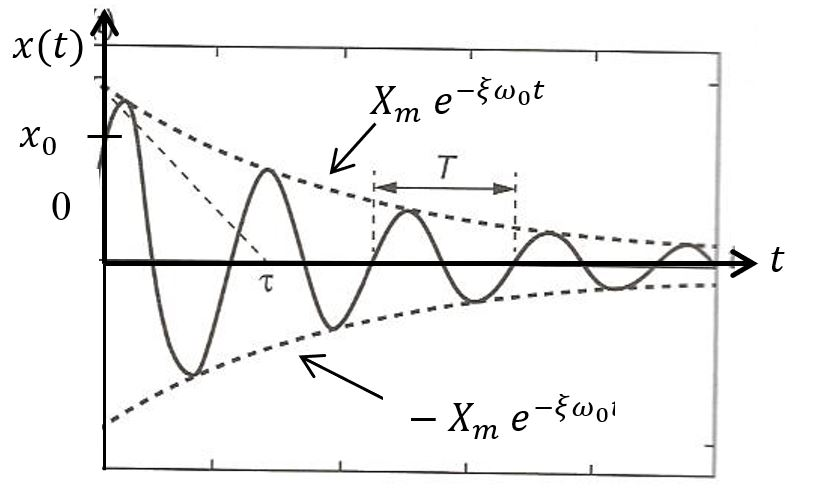
\includegraphics[width=.6\linewidth]{P1corr.jpg}
  \caption{Allure du graphe. On note la dérivée non nulle en 0.}
  \label{fig:P1corr}
\end{figure}

}

\QR
{Justifier qualitativement que l’énergie mécanique $E(t)$ est une fonction décroissante de $t$. À quoi cela est-il dû ?}
{
A cause des frottements, l’énergie mécanique $E(t)$ est une fonction décroissante de $t$.
}

\QR
{On envisage deux temps successifs $t_1$ et $t_2$ pour lesquels les déplacements sont $x_1$ et $x_2$, tels que $t_2 > t_1$ 
et $t_2-t_1=T$ , où $T$ est la période des oscillations amorties. 
En utilisant l’équation (3) et en considérant que $\xi \ll 1$, montrer que :            

\centers{$\ln{\left(\f{x_1}{x_2}\right)} \approx 2\pi\xi$}
}
{
Cela fait penser au décrément logarithmique :

\centers{
 $\delta=\ln{\f{x\left(t\right)}{x\left(t+T\right)}=\ln{\left(\f{x_1}{x_2}\right)}=\ln{\f{{X_me}^{\alpha t}\cos{\left(\W t+\varphi\right)}}{{X_me}^{\alpha(t+T)}\cos{\left(\W(T+t)+\varphi\right)}}=\ln{\left(e^{-\alpha T}\right)}}}$}
 
 \noindent
  car cosinus est une fonction périodique de période $T$.
Soit : 

\centers{$\delta=\ln{\left(\f{x_1}{x_2}\right)}=-\alpha T=\xi\w_0 T=\xi\w_0\f{2\pi}{\W}=\xi\w_0\f{2\pi}{\w_0\sqrt{1-\xi^2}}= \xi\f{2\pi}{\sqrt{1-\xi^2}}$}


Or par hypothèse,  $\xi \ll 1$ , donc $1-\xi^2\approx 1$ ; Alors

\centers{ $\ln{\left(\f{x_1}{x_2}\right)}\approx2\pi\xi$}
}

\QR
{Toujours dans le cas où $\xi\ll 1$, le relevé du déplacement horizontal de la plateforme en fonction du temps 
est représenté en figure 2 ci-dessous. En utilisant les deux points qui sont indiqués sur la figure 2, déterminer les valeurs numériques de $k$, $\xi$ et $\gamma$ (avec leurs unités). Comment ce tracé serait-il modifié si $\xi$ augmentait (un rapide graphique peut permettre d’être plus explicite) ? 

\begin{figure}[htbp!]
  \centering
  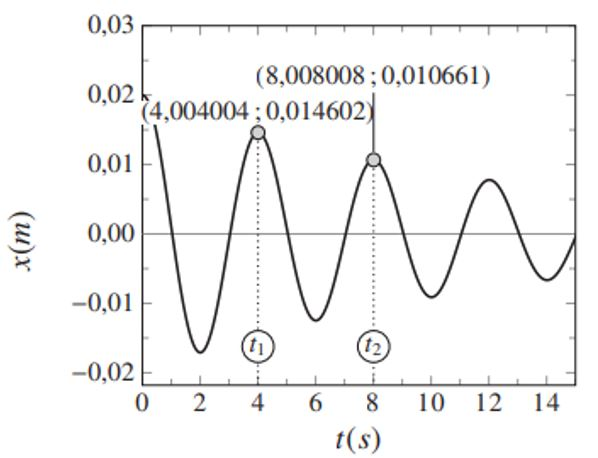
\includegraphics[width=.6\linewidth]{P2graph}
  \caption{ Relevé du déplacement horizontal $x$ (en m) de la plateforme de
  masse $m = \SI{110}{tonnes}$ en fonction du temps $t$ (en s). Les deux temps
$t_1$ et $t_2$ mentionnés en question Q6 sont indiqués.}
  \label{fig:P2graph}
\end{figure}

}
{
On lit $x_1=\SI{0,014602}{m}$ et $t_1=\SI{4,004004}{s}$, puis $x_2=\SI{0,010661}{m}$ et $t_2=\SI{8,008008}{s}$.
	D’après l’énoncé, on a  $T=t_2-t_1$ et comme $\xi \ll 1$ alors
	
 \centers{$\w_0\approx\W=\f{2\pi}{T}=\f{2\pi}{t_2-t_1}$}
	
 
 \leftcenters{ car $\W  =\w_0\sqrt{1-\xi^2}$. De plus,}{ $\w_0=\sqrt{\f{k}{m}}$}
 
\leftcenters{ Donc}{ $k=m\w_0^2=m\f{4\pi^2}{\left(t_2-t_1\right)^2} = 110.{10}^3\f{4\pi^2}{\left(8,008008-4,00400\right)^2} = \SI{2,71e5} {N.m^{-1}}$}

 \noindent
	D’autre part d’après Q6, 
	
\centers{$\ln{\left(\f{x_1}{x_2}\right)}=2\pi\xi$}
\leftcenters{Soit }{$\xi=\f{\ln{\left(\f{x_1}{x_2}\right)}}{2\pi} = \f{\ln{\left(\f{0,014602}{0,010661}\right)}}{2\pi} = \num{5,01e-2}$}
	 
\noindent
Remarque : on trouve en effet comme attendu $\xi\ll1$. C'est cohérent. 

\medskip

\leftcenters{Enfin, d’après Q1,} {$\xi=\f{\gamma}{2}\sqrt{\f{1}{mk}}$}
	
\leftcenters{Soit}{ $\gamma=2\xi\sqrt{mk} = 2\times5.01.{10}^{-2}\sqrt{110.{10}^3\times2,71.{10}^5} = \SI{1,73e4} {N.s.m^{-1}}$} .

\noindent
	Si $\xi$ augmentait, l’amortissement augmenterait, la décroissance exponentielle serait plus rapide, on 
verrait moins d’oscillations et la pseudo-pulsation $\W$  diminuerait et la pseudo-période $T={2\pi}/{\W}$ augmenterait.
}

\enonce
{
\medskip

\noindent
\underline{Outils mathématiques} : 		

\centers{$cos\left(a+b\right)=\cos{\left(a\right)}\cos{\left(b\right)}-\sin{\left(a\right)}\sin(b) \quad \text{et} \quad
					{cos}^2\left(\alpha\right)+{sin}^2\left(\alpha\right)=1$} 
}

\end{document}
